%%%%%%%%%%%%%%%%%%%%%%%%%%%%%%%%%%%%%%%%%%%%%%%%%%%%%%%%%%%%%%%%%%%%%%%%%%%%%%%%%%%%%%%%%%%%%%%%%%%%%%%%%%%%%%%%%%%%%%%%%%%%%%%%%%%%%%%%%%%%%%%%%%%%%%%%%%%
% Supplementary material for: Conversational Speech for Respiratory Triage in Primary Care: A Pilot Study
%%%%%%%%%%%%%%%%%%%%%%%%%%%%%%%%%%%%%%%%%%%%%%%%%%%%%%%%%%%%%%%%%%%%%%%%%%%%%%%%%%%%%%%%%%%%%%%%%%%%%%%%%%%%%%%%%%%%%%%%%%%%%%%%%%%%%%%%%%%%%%%%%%%%%%%%%%%

\documentclass[utf8]{frontiers_suppmat} % for all articles
\usepackage{url,hyperref,lineno,microtype}
\usepackage[onehalfspacing]{setspace}
\usepackage{graphicx}
\usepackage{booktabs}
\usepackage{xcolor}

% Review-comment command: \comment{your note here} renders inline in magenta as [COMMENT: your note here]
\newcommand{\comment}[1]{\textcolor{magenta}{[COMMENT: #1]}}

% Leave a blank line between paragraphs instead of using \\

\begin{document}
\onecolumn
\firstpage{1}

\title[Supplementary Material]{{\helveticaitalic{Supplementary Material}}}


\maketitle


\section{Data distribution of the analytic sample}
\label{supp:data-distribution}

The analytic sample comprises 514{,}381 visits from 379{,}227 unique adult patients. The following subsections describe its demographic, geographic, clinical, and audio-duration distributions.

\subsection{Demographic distribution}
\label{supp:demographic}

Median patient age at the time of visit is 38 years, with an interquartile range of 28 to 55 years and a mean of 42.7 years. The age range spans 18 to 106 years. The distribution is right-skewed (Figure~\ref{supp_fig_demographics}A), peaking in the 25 to 29 bin and decaying monotonically thereafter. Sex distribution is 63.5\% female (326{,}412 visits) and 36.5\% male (187{,}884 visits), with 72 visits recorded as Unknown and 9 as Other. The female skew is consistent with primary care utilization patterns reported in US ambulatory care surveys [TODO: CITE source, e.g., CDC NAMCS] and is not a recruitment artifact of this work. Patient-level deduplication (n=379{,}227) yields the same median age (38), an interquartile range of 28 to 55, and a sex distribution within 0.1\% of the visit-level numbers, indicating that the visit-level view is not distorted by a small number of high-frequency patients. The longitudinal structure of the sample is sparse (Figure~\ref{supp_fig_demographics}B): 77.1\% of patients (n=292{,}422) contributed a single visit, 15.4\% (n=58{,}322) contributed two, 6.9\% (n=26{,}328) contributed three to five, and 0.5\% (n=2{,}064) contributed six to ten. A small tail of 89 patients (0.02\%) contributed between 11 and 25 visits, and no patient in the sample exceeded 25 visits.

\begin{figure}[h!]
\begin{center}
\begin{minipage}[t]{0.48\linewidth}
\centering
\textbf{(A)}\\
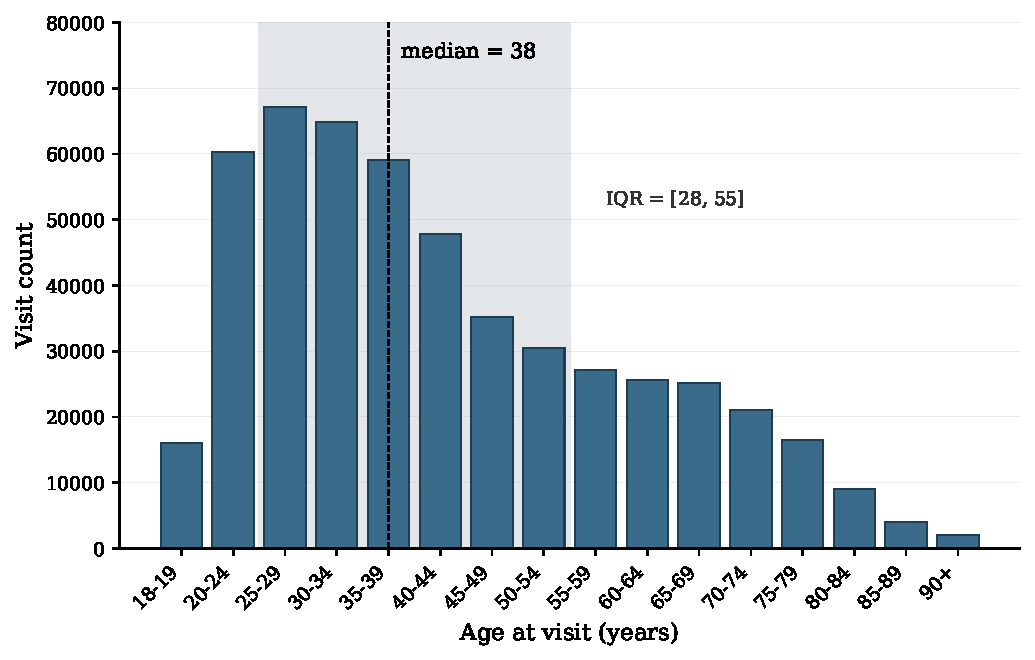
\includegraphics[width=\linewidth]{fig_demographics_age}
\end{minipage}\hfill
\begin{minipage}[t]{0.48\linewidth}
\centering
\textbf{(B)}\\
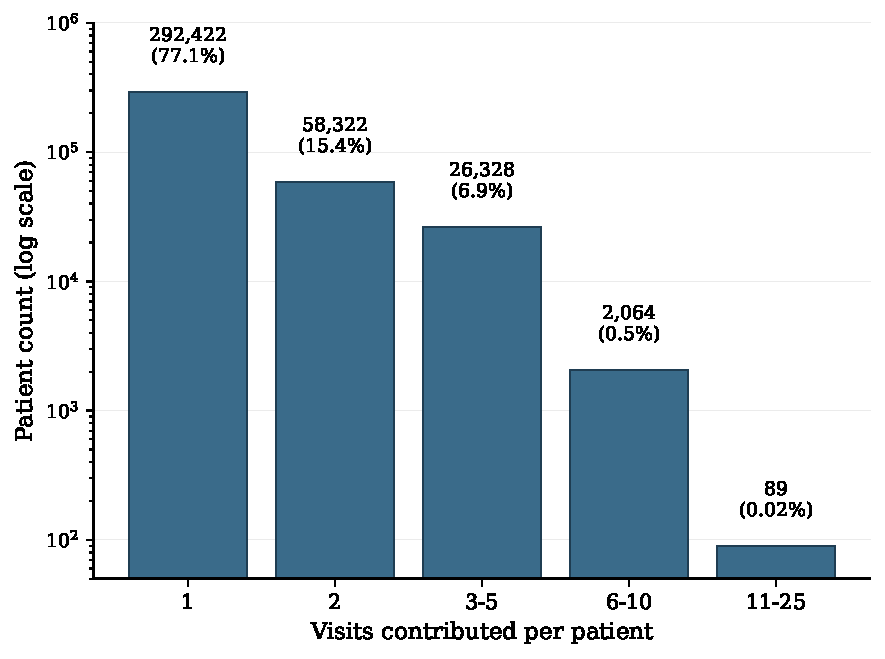
\includegraphics[width=\linewidth]{fig_demographics_visits_per_patient}
\end{minipage}
\end{center}
\caption{Demographic distribution of the analytic sample (n=514{,}381 visits from 379{,}227 unique patients). \textbf{(A)} Patient age distribution at the time of visit, binned in 5-year intervals; the distribution is right-skewed and peaks in the 25 to 29 bin. \textbf{(B)} Visits-per-patient distribution; 77.1\% of patients contributed a single visit and no patient contributed more than 25.}
\label{supp_fig_demographics}
\end{figure}

\subsection{Geographic distribution}
\label{supp:geographic}

Geographic information is recorded at the patient level as the state and city of the patient's address. The analytic sample spans all 50 US states, the District of Columbia, and four US territories (Puerto Rico, the US Virgin Islands, Guam, and the Northern Mariana Islands), with a small number of visits also recorded from US military addresses and from international jurisdictions where the network's patients were temporarily resident. State and city fields were normalized prior to the analysis below: full-name spellings of states were merged into their two-letter codes, and visits with unparseable state values (single characters, punctuation, numeric sentinels, and similar artifacts, totaling approximately 0.17\% of the sample) were excluded from the geographic counts but retained in all other analyses. The resulting distribution is heavily concentrated in California and the Northeast (Figure~\ref{supp_fig_geography}A): California alone accounts for 58.4\% of visits (n=300{,}229), followed by New Jersey at 15.6\% (n=80{,}350), Arizona at 5.3\% (n=27{,}383), Washington at 4.2\% (n=21{,}348), and Massachusetts at 3.4\% (n=17{,}571). These five states together account for 86.9\% of the sample, and the top ten states account for 95.3\%. At the city level, the sample spans 9{,}251 unique cities, with the most heavily represented being Los Angeles, San Francisco, Tucson, San Jose, and Simi Valley (Figure~\ref{supp_fig_geography}B). The long tail is substantial: 3{,}800 cities (41\% of unique cities) contributed a single visit each.

\begin{figure}[h!]
\begin{center}
\begin{minipage}[t]{0.48\linewidth}
\centering
\textbf{(A)}\\
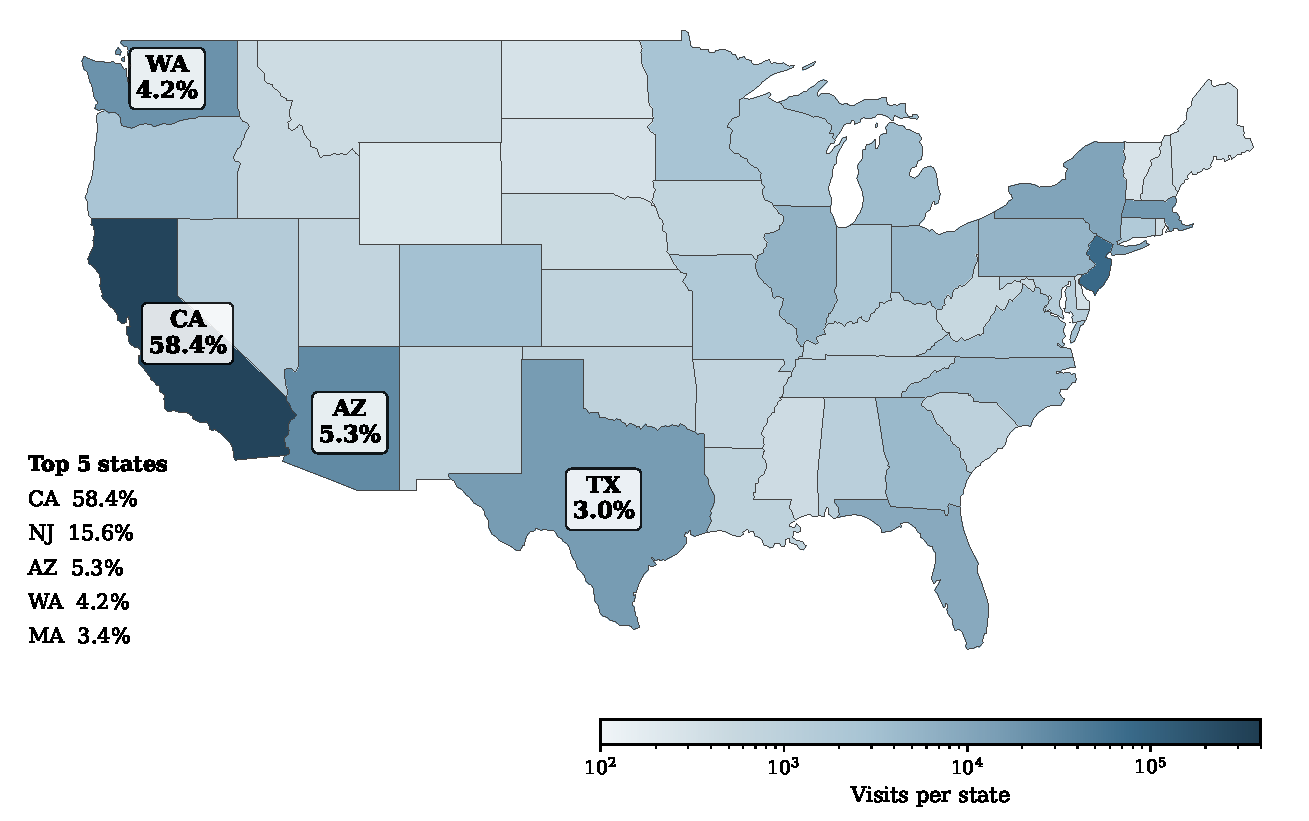
\includegraphics[width=\linewidth]{fig_geography_states}
\end{minipage}\hfill
\begin{minipage}[t]{0.48\linewidth}
\centering
\textbf{(B)}\\
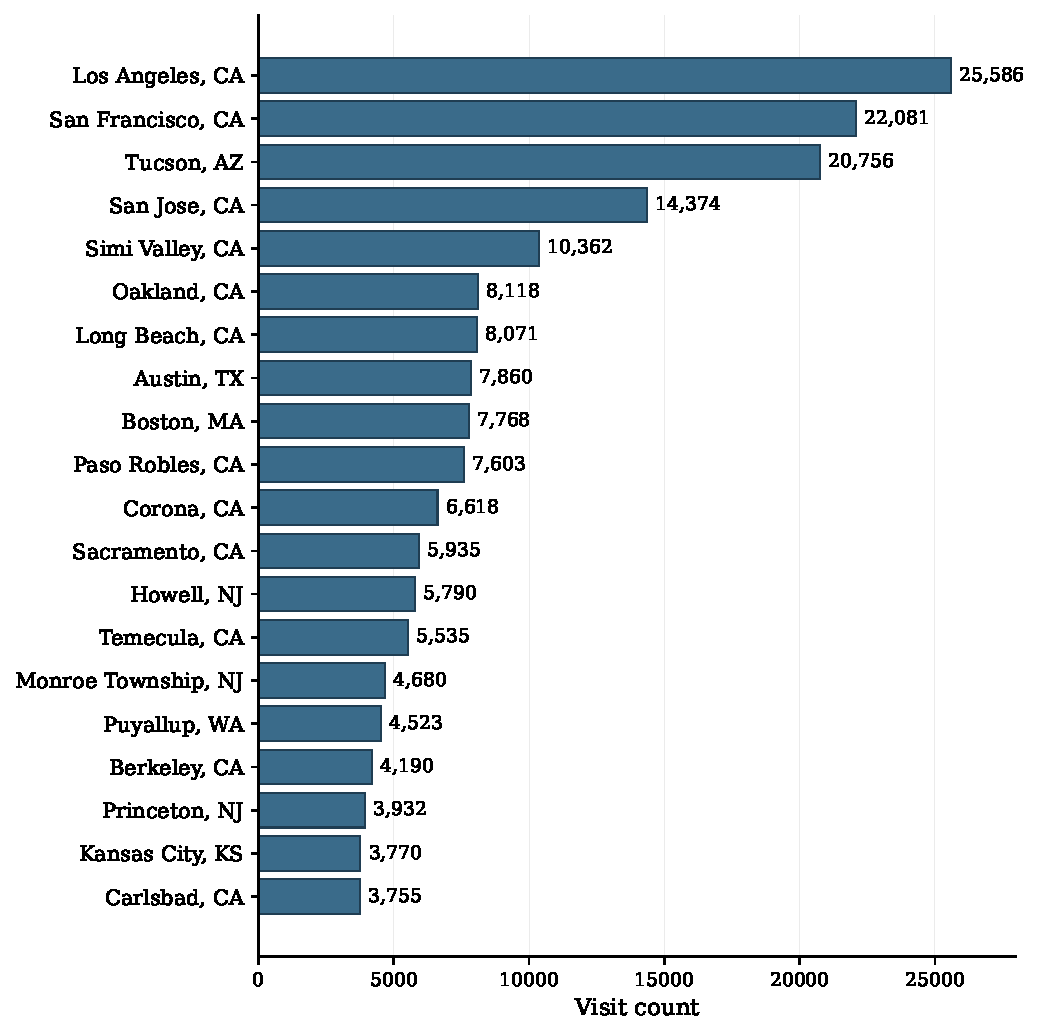
\includegraphics[width=\linewidth]{fig_geography_cities}
\end{minipage}
\end{center}
\caption{Geographic distribution of the analytic sample (n=514{,}381 visits from 379{,}227 unique patients). \textbf{(A)} State-level visit counts; California accounts for 58.4\% of visits and the top five states (California, New Jersey, Arizona, Washington, Massachusetts) account for 86.9\%. \textbf{(B)} City-level visit distribution across 9{,}251 unique cities; the long tail comprises 3{,}800 cities (41\%) that contribute a single visit each.}
\label{supp_fig_geography}
\end{figure}

\subsection{Clinical distribution}
\label{supp:clinical}

The clinical composition of the analytic sample is summarized by the distribution of primary ICD-10 diagnosis codes assigned to each visit. At the chapter level, respiratory diagnoses (Chapter J) account for 52.3\% of all primary codes (Figure~\ref{supp_fig_clinical}A), which is the direct consequence of the cohort construction described in the main paper: visits are included in the analytic sample if and only if they satisfy the inclusion or exclusion criteria of at least one of the 11 binary classification tasks, and most of those tasks anchor on respiratory ICD-10 codes. The non-respiratory share is dominated by symptoms and signs (Chapter R, 12.74\%), musculoskeletal complaints (Chapter M, 10.64\%), genitourinary visits (Chapter N, 8.49\%), and skin conditions (Chapter L, 6.20\%). The U chapter (special purposes), which contains the U07.1 code for confirmed COVID-19, contributes 2.92\%. All remaining chapters together account for less than 7\% of visits. This distribution reflects the analytic sample, not the originating primary care population at large; the upstream selection into the 11 binaries deliberately enriches for respiratory presentations and for non-respiratory acute-illness negatives.

At the individual-code level (Figure~\ref{supp_fig_clinical}B), the analytic sample is dominated by acute upper respiratory presentations. J06.9 (acute upper respiratory infection, unspecified) alone accounts for 19.74\% of all visits, followed by J02.9 (acute pharyngitis, unspecified) at 9.33\%. Sinusitis codes (J01.90 and J01.00) together contribute 8.43\%. The top 20 primary codes (each representing at least 1\% of visits) collectively account for 71.07\% of the analytic sample. Notable non-respiratory codes in the top 20 are N39.0 (urinary tract infection, 7.34\%), N30.01 (acute cystitis with hematuria, 1.31\%), R30.0 (dysuria, 1.62\%), M54.50 (low back pain, 1.67\%), R10.9 (unspecified abdominal pain, 1.07\%), and R07.0 (pain in throat, 1.17\%); these visits are present in the analytic sample because they serve as acute non-respiratory negative controls for one or more of the binary classification tasks. The prominence of ``unspecified'' codes (J06.9, J02.9, J01.90, J22, J18.9, J20.9, R10.9, R07.0, J45.901) reflects the reality of primary care coding, where clinicians frequently assign the least-specific code consistent with the presentation.

Patient-level documentation of chronic conditions and comorbidities is available for the analytic sample through the full ICD-10 code arrays attached to each patient's visit history. Documented prevalences across the analytic sample of 379{,}227 patients are 4.69\% for chronic respiratory disease (defined as any occurrence of J44, J45, J47, J84, or E84), 1.35\% for anxiety (F41), 0.93\% for gastroesophageal reflux disease (K21), 0.59\% for depression (F32 or F33), 0.33\% for obesity (E66), 0.12\% for tobacco use or dependence (F17, Z72.0, or Z87.891), 0.09\% for obstructive sleep apnea (G47.3x), and 0.04\% for heart failure (I50). These prevalences are computed against the full denominator of 379{,}227 patients, treating absence of the code as absence of the condition. They are therefore documentation prevalences rather than true population prevalences, and they undercount by construction: a condition that exists but has not been coded during any visit in the observation window does not contribute. The tobacco use figure of 0.12\% is the clearest example, since US adult tobacco use prevalence is approximately 14\% [TODO: CITE source, e.g., CDC NHIS or BRFSS], and the present figure is best read as a coding-rate floor rather than a true-prevalence estimate.

\begin{figure}[h!]
\begin{center}
\begin{minipage}[t]{0.48\linewidth}
\centering
\textbf{(A)}\\
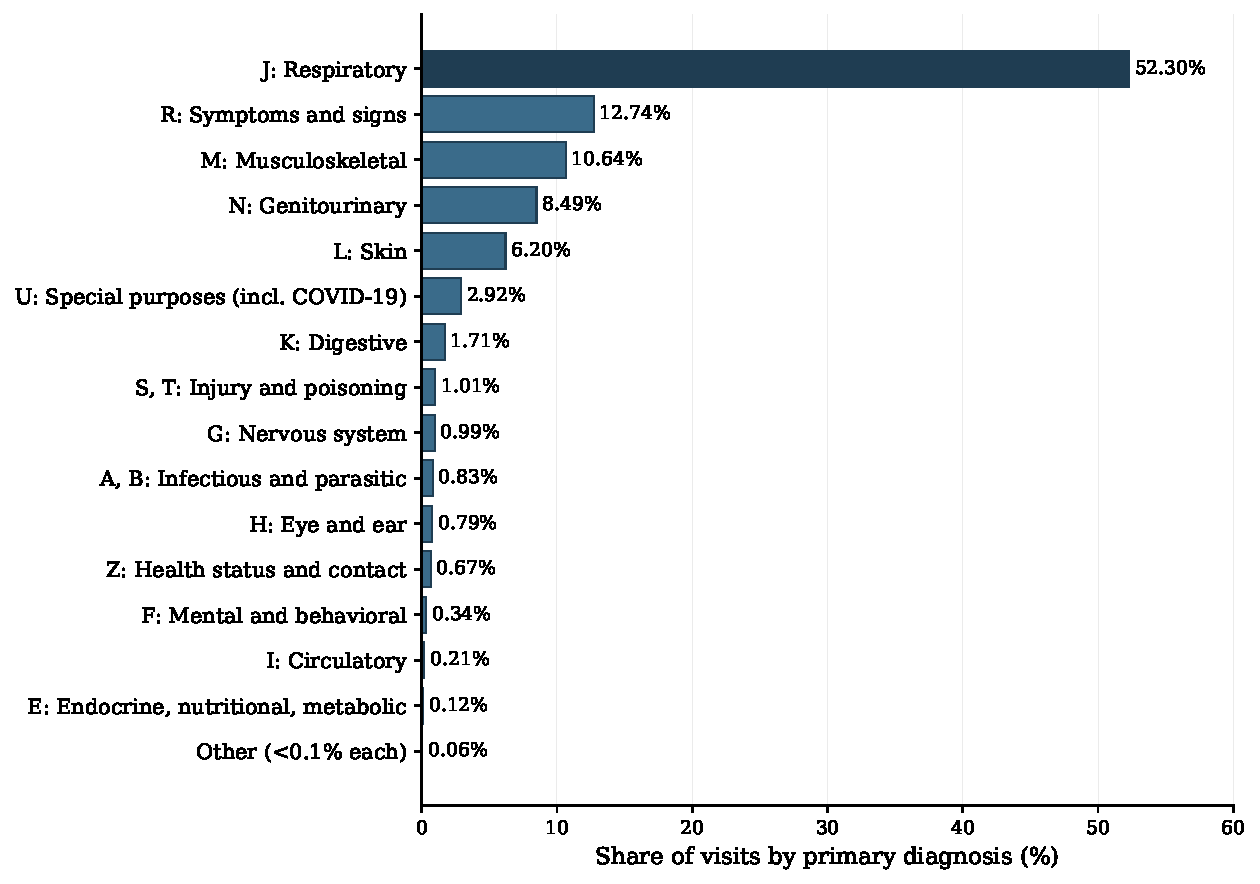
\includegraphics[width=\linewidth]{fig_clinical_chapters}
\end{minipage}\hfill
\begin{minipage}[t]{0.48\linewidth}
\centering
\textbf{(B)}\\
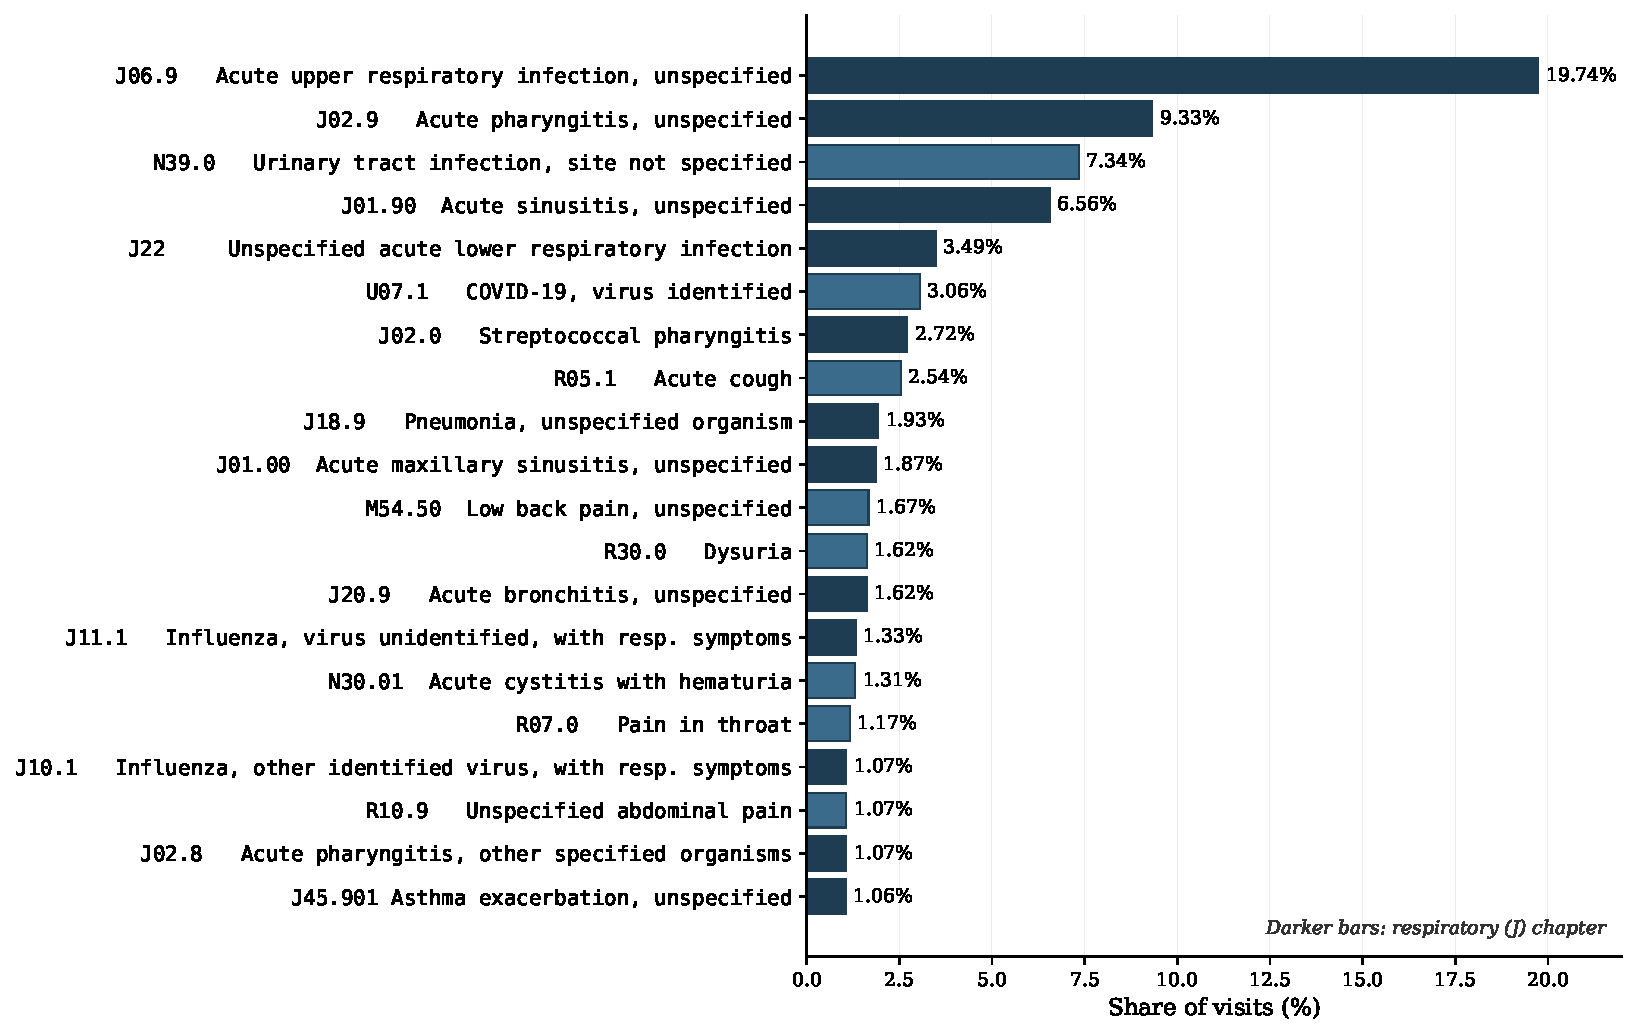
\includegraphics[width=\linewidth]{fig_clinical_top_codes}
\end{minipage}
\end{center}
\caption{Clinical distribution of primary ICD-10 codes across the analytic sample (n=514{,}381 visits from 379{,}227 unique patients). \textbf{(A)} ICD-10 chapter distribution; the respiratory chapter (J) accounts for 52.3\% of primary diagnoses, followed by symptoms and signs (R, 12.74\%), musculoskeletal (M, 10.64\%), genitourinary (N, 8.49\%), and skin (L, 6.20\%). \textbf{(B)} Top primary ICD-10 codes; the top 20 codes account for 71.07\% of visits, led by J06.9 (acute upper respiratory infection, unspecified) at 19.74\% and J02.9 (acute pharyngitis, unspecified) at 9.33\%.}
\label{supp_fig_clinical}
\end{figure}

\subsection{Audio duration distribution}
\label{supp:audio-duration}

Patient audio duration is the length of the patient-channel signal extracted from each recording by the diarization pipeline described in the main paper; it is the input length to the feature extractor for that visit. Across the 514{,}381 visits in the analytic sample, the median duration is 27.8 seconds with an interquartile range of 15.4 to 47.2 seconds, the mean is 36.8 $\pm$ 34.1 seconds, and the range is 0.7 to 776 seconds (Figure~\ref{supp_fig_duration}). The distribution is unimodal and right-skewed on a linear scale; on the log scale of Figure~\ref{supp_fig_duration} it appears roughly symmetric. A small accumulation near the one-second boundary corresponds to a minor leak in the audio-quality filter, where 3{,}542 visits (0.7\%) recorded a duration below the nominal one-second floor; this leak is too small to bias any downstream analysis but we note it for transparency. The total measured patient audio across the analytic sample is 5{,}033 hours, representing the largest collection of real-world conversational primary care audio reported to date for the purpose of acoustic respiratory triage.

\begin{figure}[h!]
\begin{center}
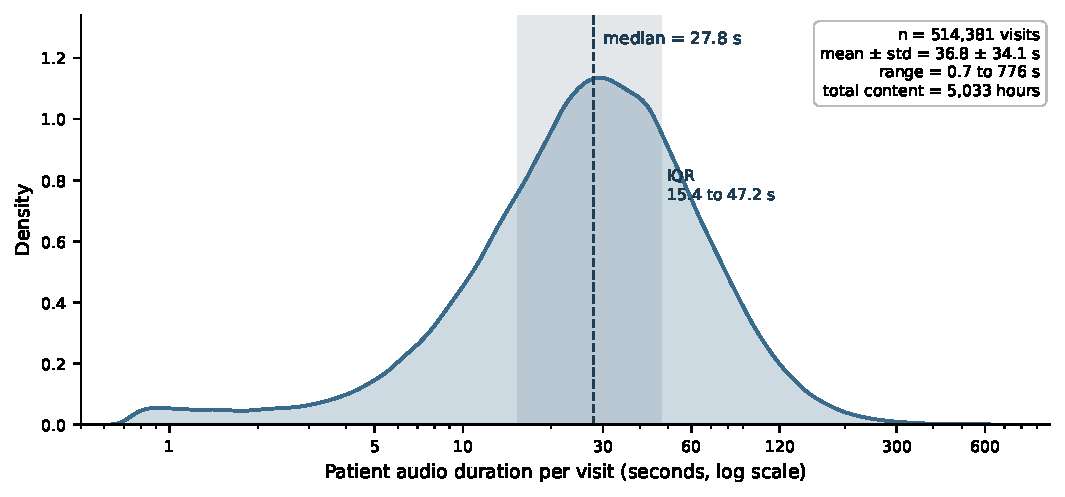
\includegraphics[width=\linewidth]{fig_duration}
\end{center}
\caption{Patient-channel audio duration across the analytic sample (n=514{,}381 visits). The distribution is unimodal and right-skewed on a linear scale (median 27.8 s, interquartile range 15.4 to 47.2 s, mean 36.8 $\pm$ 34.1 s, range 0.7 to 776 s); on the log scale shown here it appears roughly symmetric. The total measured patient audio is 5{,}033 hours.}
\label{supp_fig_duration}
\end{figure}


\section{Modeling and evaluation details}
\label{supp:modeling}

\subsection{Diarization configuration}
\label{supp:diarization}

The full-recording audio for each visit is submitted to Google Cloud Speech-to-Text v2 using the Chirp 3 acoustic model in its BatchRecognize mode, with one to two expected speakers, English as the recognition language, and word-level timestamps as the output granularity. Words from consecutive same-speaker positions are merged into per-speaker segments, with speaker labels normalized to SPEAKER\_01 and SPEAKER\_02. To identify which of the diarized speakers is the patient, the diarized transcript is passed to the gemini-flash-3.1-lite large language model with a deterministic system prompt that asks for the speaker label of the primary subject of the visit, defined as the patient or person under evaluation rather than a caregiver, translator, automated system, or any other participant. The classifier returns either a speaker label or a sentinel value indicating that no patient is present in the recording, in which case the visit is excluded from the pipeline. Patient-only audio is then reconstructed by concatenating, in chronological order, the time-aligned slices of the original recording corresponding to the chosen speaker label, producing a single contiguous WAV file containing only the patient's voice.

The signal entering feature extraction is the patient-only WAV at the rate produced by the diarization pipeline (16 kHz). When the source audio is stereo or multi-channel, channels are averaged to mono before processing; the source data for this work is single-channel by construction. No loudness or amplitude normalization, no denoising, no voice activity detection beyond the diarization-based speaker labels, and no silence trimming beyond the segment-level cuts produced by diarization are applied.

\subsection{Feature extraction details}
\label{supp:feature-extraction}

One set of six streams is composed of 88 features that are produced by the openSMILE eGeMAPSv02 Functionals feature set (computed at 16 kHz sampling rate using the published eGeMAPSv02 configuration of frame-level low-level descriptors aggregated into clip-level functionals such as mean, normalized standard deviation, percentiles, percentile ranges, and rising and falling slope statistics). The 88 outputs are partitioned into six streams aligned with the components of the speech production apparatus: pitch (10 features, F0-based), loudness (10 features, perceptual loudness statistics), spectral (28 features including MFCC1 to MFCC4 [Mel-frequency cepstral coefficients], spectral flux, the Hammarberg index, and voiced and unvoiced spectral slopes), voice quality (10 features covering jitter, shimmer, and harmonics-to-noise ratio), formants (18 features covering F1, F2, and F3 frequencies, bandwidths, and amplitudes relative to F0), and temporal (12 features including voiced and unvoiced segment statistics, loudness peaks per second, and equivalent sound level).

One stream contains 281 features derived from librosa (version 0.11.0), summarizing seven families of low-level descriptors over the whole patient clip: Mel-frequency cepstral coefficients (13 bands with nine summary statistics each), chromagram (12 pitch classes with nine statistics each), spectral descriptors (centroid, bandwidth, contrast, flatness, rolloff, zero-crossing rate), energy features (root-mean-square), spectral contrast, tonnetz on the harmonic component, and rhythm features (tempo and predominant local pulse). Librosa frame-level extraction uses the library defaults of a 2048-sample FFT window, a 512-sample hop, and a 2048-sample analysis window, which at the 16 kHz sampling rate corresponds to a 128 ms window and 32 ms hop. Each per-frame low-level descriptor is summarized into nine statistics (mean, standard deviation, minimum, maximum, median, 25th and 75th percentiles, interquartile range, and range), and single-scalar features such as tempo are stored directly.

One stream contains 24 features derived from a valence, arousal, and dominance predictor (WavLM-VAD-Odyssey2024), computed as per-clip distribution statistics of the three predicted axes. One stream contains 19 features from a temporal-analysis extractor that combines praat-parselmouth syllable-and-pause detection (yielding total syllables, total pauses, total file duration, phonation time, speech rate, articulation rate, average syllable duration, total pause duration, and maximum, minimum, and mean pause durations) with librosa tempo statistics (mean, median, standard deviation, minimum, maximum, interquartile range, coefficient of variation, and range).

Non-numeric columns and extraction-metadata columns are dropped at the consolidation step, and visits whose source feature parquet is missing one or more required columns are dropped at compact-build time; this affects approximately three to five percent of the visits per binary and is recorded in a sidecar audit file.

\subsection{Model architecture details}
\label{supp:model-architecture}

The nine feature streams are concatenated in a fixed order (valence-arousal-dominance, pitch, loudness, spectral, voice quality, formants, temporal, temporal analysis, librosa) before being passed to the network. The network consists of two to four hidden blocks followed by a final linear projection to a single output logit. Each hidden block is a sequence of a linear layer, a one-dimensional batch normalization, a GELU activation, and a dropout layer with rate 0.5. The final linear layer projects the last hidden block's activations to a single logit, with no activation; sigmoid is applied at inference time when probabilities are required.

\subsection{Training hyperparameters}
\label{supp:training-hyperparameters}

For each binary, balancing reduces the analytic sample to twice the size of the minority class. The minority class is taken in full at the visit level. The majority class is downsampled by sampling unique patients without replacement until the expected visit count matches the minority size; if the realized visit count exceeds the target, the class is trimmed to exact size at the visit level. Sampling is seeded for reproducibility.

Each model is trained for up to 50 epochs with AdamW (weight decay 0.001), a cosine-annealing learning rate schedule with no warmup, and gradient norm clipping at 1.0. The minibatch size is 256. Training halts early when development loss has not improved for 10 consecutive epochs, and the checkpoint with the lowest development loss is retained as that fold's final model.

The learning rate and the hidden-layer topology are chosen per binary by a grid search over four learning rates (1e-4, 3e-4, 1e-3, 3e-3) and four candidate topologies (two-block at 128 and 64; three-block at 256, 128, 64; four-block at 256, 128, 64, 32; three-block at 512, 256, 128), yielding 16 combinations per binary. Each combination is trained once on a single development split of the balanced cohort, and the combination achieving the lowest development loss is selected. The selected combination is then retrained under five-fold cross-validation, producing five fold-specific models.

\end{document}
